\documentclass[sigplan]{acmart}
\usepackage{booktabs} % For formal tables


%\setcopyright{acmcopyright}
% Load basic packages
\usepackage{balance}       % to better equalize the last page
\usepackage{graphics}      % for EPS, load graphicx instead 
\usepackage[T1]{fontenc}   % for umlauts and other diaeresis
\usepackage{txfonts}
\usepackage{mathptmx}
%\usepackage[pdflang={en-US},pdftex]{hyperref}
\usepackage{color}
\usepackage{booktabs}
\usepackage{textcomp}

% Some optional stuff you might like/need.
\usepackage{microtype}        % Improved Tracking and Kerning
% \usepackage[all]{hypcap}    % Fixes bug in hyperref caption linking
\usepackage{ccicons}          % Cite your images correctly!
% \usepackage[utf8]{inputenc} % for a UTF8 editor only

% Custom packages

\usepackage{paralist}
\usepackage{enumitem}

\usepackage{tikz}
\usetikzlibrary{shadows,shapes}
\usepackage{pgfplots}
\pgfplotsset{compat=1.10}

\usepackage{xcolor}
\usepackage{colortbl}
\definecolor{Gray}{gray}{0.90}

\usepackage{algorithm}
\usepackage{algorithmicx}
\usepackage{algpseudocode}

% If you want to use todo notes, marginpars etc. during creation of
% your draft document, you have to enable the "chi_draft" option for
% the document class. To do this, change the very first line to:
% "\documentclass[chi_draft]{sigchi}". You can then place todo notes
% by using the "\todo{...}"  command. Make sure to disable the draft
% option again before submitting your final document.
\usepackage[textsize=tiny, textwidth=1.5cm]{todonotes}
\newcommand{\TODO}[1]{\todo[inline]{#1}}
\newcommand{\Abhishek}[1]{\todo[color=yellow!50, linecolor=black!50]{\textbf{Abhishek}: #1}}
\newcommand{\Aron}[1]{\todo[color=green!40, linecolor=black!50]{\textbf{Aron}: #1}}
\newcommand{\AronInline}[1]{\todo[inline,size=\small,color=green!40, linecolor=black!50]{\textbf{Aron}: #1}}
\newcommand{\Doug}[1]{\todo[color=red!40, linecolor=black!50]{\textbf{Doug}: #1}}
\newcommand{\Jonatan}[1]{\todo[color=gray!40, linecolor=black!50]{\textbf{Jon}: #1}}
\newcommand{\JonInline}[1]{\todo[inline,size=\small,color=gray!40, linecolor=black!50]{\textbf{Jon}: #1}}

%\usepackage[normalem]{ulem}
%\newcommand{\change}[2]{\textcolor{red}{\sout{#1}} \textcolor{blue}{#2}}
\newcommand{\change}[2]{#2} % DO NOT DISPLAY CHANGES

\newcommand{\circled}[1]{\tikz[baseline=(char.base)]{\node[shape=circle, draw, inner sep=0.5pt, solid] (char) {#1};}}
            
\newcommand{\field}[1]{\texttt{#1}}


% llt: Define a global style for URLs, rather that the default one
\makeatletter
% \def\url@leostyle{%
%   \@ifundefined{selectfont}{
%     \def\UrlFont{\sf}
%   }{
%     \def\UrlFont{\small\bf\ttfamily}
%   }}
\makeatother
\urlstyle{leo}

\acmConference[SERIAL '17]{SERIAL 2017}
              {December 2017}{Las Vegas, Nevada USA} 
\acmYear{2017}
\copyrightyear{2017}

% create a shortcut to typeset table headings
% \newcommand\tabhead[1]{\small\textbf{#1}}

% End of preamble. Here it comes the document.
\begin{document}

% TODO: remove before submission, added only for todonotes
\setlength{\marginparwidth}{1.5cm}

%\allowdisplaybreaks

\title[Anonymity in Blockchain-Based Transactive Microgrids]{On the Design of Communication and Transaction Anonymity in Blockchain-Based Transactive Microgrids}

\author{Jonatan Bergquist}
\affiliation{\institution{Datarella GmbH}}
\author{Aron Laszka}
\affiliation{\institution{Vanderbilt University}}
\author{Monika Sturm}
\affiliation{\institution{Siemens Corporate Technology}}
\author{Abhishek Dubey}
\affiliation{\institution{Vanderbilt University}}

\renewcommand{\shortauthors}{J. Bergquist et al.}


%\Aron{We need to add authors (\url{https://serial17.ibr.cs.tu-bs.de/cfp.html}: ``Reviewing is single-blind.'')}

\begin{abstract}
%\textcolor{red}{The abstract needs to be rewritten}
%Transactive microgrids are emerging as the next  advancement for power grid. They provide robust capabilities for integrating distributed generation resources in communities, creat
 Transactive microgrids are emerging as a transformative solution for the problems faced by distribution system operators due to an increase in the use of distributed energy resources and a rapid acceleration in renewable energy generation, such as wind and solar power. Distributed ledgers have recently found widespread interest in this domain due to their ability to provide transactional integrity across decentralized computing nodes. However, the existing state of the art has not focused on the privacy preservation requirement of these energy systems --  the transaction level data can provide much greater insights into a prosumer's behavior compared to smart meter data. %\Aron{We could also mention safety requirements as a challenge to privacy (for stable grid control, we need to disseminate information).}\Jonatan{Resolved} 
 There are specific safety requirements in transactive microgrids to ensure the stability of the grid and to control the load. To fulfil these requirements, the distribution system operator needs transaction information from the grid, which poses a further challenge to the privacy goals. This problem is made worse by requirement for off-blockchain communication in these networks. In this paper, we extend a recently developed trading workflow called PETra and describe our solution for communication and transactional anonymity.    
 %exacerbated further by consideration that 
 %Blockchains is an emerging technology that has found widespread interest in this domain  These, on one hand, pose a decentralized power system controls problem, requiring strategic microgrid control to maintain stability for the community and for the utility. On the other hand, they require robust financial markets where transactions beneficial for the grid should be incentivized, while ensuring that erroneous transactions cannot destabilize the grid. 
% Successful setup and operation of these microgrids require a distributed transactive and control platform that works together to ensure that transactions of energy (a) are unforgeable in the sense that producers should not be able to create a transaction without actually producing energy, (b) are tamper proof, and (c) preserve the anonymity of the actors.
 % This last point is crucial because  the transaction level data can provide much greater insights into a prosumer's behavior compared to smart meter data. \Aron{This is the first mention of blockchains. If we are targeting SERIAL, then I think that the abstract needs to be more focused on blockchains and distributed ledgers. Maybe include them in the title as well?} In this paper, we first describe the use of blockchains to create a transactional workflow that satisfy the first two requirements. The third requirement are met by 
 
% Power grids are undergoing major changes due to rapid growth in renewable energy resources and improvements in battery technology. Significant challenges to manage the increasing complexity of these systems are the consequence. Emerging solutions arrange local communities into transactive microgrids, based on connected devices networked over a decentralized Internet-of-Things (IoT). Within a transactive microgrid, 'prosumers' (i.e., consumers with energy generation and storage capabilities) can trade energy with each other, thereby smoothing the load on the main grid using local supply. Security and safety issues that arise are protecting prosumers' personal information and secure the system from careless or malicious trading, which could destabilize the entire grid. This paper describes Privacy-preserving Energy Transactions (PETra), which is a secure and safe solution for transactive microgrids that enables consumers to trade energy without sacrificing their privacy. PETra builds on distributed ledgers, such as blockchains, and provides anonymity for communication, bidding, and trading.    
\end{abstract}

% TODO!


\keywords{transactive energy platforms, blockchain, distributed ledger, privacy, anonymity, onion routing, zero-knowledge proofs}
\maketitle

%!TEX root = paper.tex
\section{Introduction}


Transactive energy models have been proposed as a set of market based mechanisms for balancing the demand and generation of energy in communities \cite{kok2016society,cox2013structured,melton2013gridwise}.
 In this approach, customers on the same feeder (i.e. sharing a power line link) can operate in an open market, trading and exchanging generated energy locally. Distribution System Operators can be the custodian of this market, while still meeting the net demand \cite{7462854}. Blockchains have  recently emerged as a foundation for enabling the transactional service in the microgrids. For example, the Brooklyn Microgrid
(\url{brooklynmicrogrid.com}) is a peer-to-peer market for locally
generated renewable energy, which was developed by LO3 Energy as a pilot project. Similarly, RWE, and Grid Singularity have developed blockchain based solutions for incentivizing neighbors to sell excess energy to the grid and payments for electric car charging %and (c) enabling pre-paid transactions for electric bills in South Africa, respectively. 
However, those solutions do not address the requirements for off-blockchain communication network and the requirements for privacy. 
 
 
 %Due to a number of challenges, however, these services have been restricted in the present to some pilot programs like Demand/Response \cite{7462854}.  On one hand, transactive energy is a decentralized power system controls problem \cite{7452738}, requiring strategic microgrid control to maintain the stability of the community and the utility. On the other hand, it is a distributed market problem where erroneous as well as malicious transactions can create a gap between demand and supply, eventually destabilizing the system.  Furthermore, this system inherently induces a distributed  infrastructure comprised of smart meters, feeders, smart inverters, utility substations, the utility central offices, and the transmission system operator, which has to provide the necessary computation fabric to support the interplay between the energy control and the fiscal market challenges.
 
 

Specifically, while blockchains provide the necessary ledger services, we still need a  communication network for sending control commands from the DSO to the prosumers as well as initiating the trade matching mechanisms.
%as described by our recent publication \textcolor{red}{\cite{Laszka17}}. 
Additionally, this communication network and the blockchain itself must preserve the privacy of the prosumers. Energy usage patterns (actual or predicted) are sensitive, personally identifiable data. Legal requirements and security considerations make it mandatory to provide a mechanism to hide the identities and transaction patterns of trade partners. Additionally, solutions must also satisfy security and safety requirements, which often conflict with privacy goals. For example, to prevent a prosumer from destabilizing the system through careless or malicious energy trading, a transactive grid must check all of the prosumer's transactions. In a decentralized system, these checks require disseminating information, which could be used to infer the prosumer's future energy consumption. 

%This paper first describes mechanisms to implement anonymity in both the communication and transactional dimensions 

In \cite{Laszka17}, we introduced {\it Privacy-preserving Energy Transactions
(PETra)}, which is our distributed-ledger based solution that
(1) enables trading energy futures in a secure and verifiable
manner, (2) preserves prosumer privacy, and (3) enables distribution system operators to regulate trading and enforce the safety rules. In this paper, we  extend the communication and transaction anonymity mechanisms. The key contributions of this paper are (a) a survey of the key concepts required for implementing the anonymity across the two dimensions, (b) a discussion on the threats that must be considered when we implement the anonymization mechanisms, and lastly (c) a discussion on implementing the anonymization extensions in PETra. 
%This paper describes privacy-aspects of the communication and transactional components of transactive microgrids. Specifically, we analyze two existing schemes for communication anonymity and two schemes for transaction anonymity. They are analyzed with respect to security and known attacks. The schemes are also judged for appropriateness in regards to their application in transactive microgrids. Based on the analysis, we propose a novel design for achieving communication and transaction anonymity in transactive microgrids.
% REDUNDANT OUTLINE
% The outline of this paper is as follows. We first summarize the transaction workflow described in \cite{Laszka17}. Thereafter, we focus on the key contributions of this paper, a discussion on the privacy challenges for both communication as well as transactions.  

% This paper introduces Privacy-preserving Energy Transactions (PETra), which is our distributed-ledger based solution that (1) enables trading energy futures in a secure and verifiable manner, (2) preserves prosumer privacy, and (3) enables DSOs to regulate trading and enforce certain safety rules. 

The outline of this paper is as follows. We first present an overview of the PETra workflow described in \cite{Laszka17} in Section \ref{sec:petra}. We then discuss the communication anonymity extensions in Section \ref{comm} and transaction anonymity in Section \ref{trans}. Section \ref{commthreat} discusses the threat vectors for the communication anonymity approach. Section \ref{transthreat} describes the transaction anonymity threats.
Finally, we provide concluding remarks in Section~\ref{sec:discussion}.

\section{Preliminaries and Requirements}

\subsection{Transactive Microgrid Components}

Here, we describe a basic system model of transactive microgrids.
We discuss the following components: a distributed ledger for recording transactions, a bid storage service that facilitates finding trade partners, a microgrid controller for regulating the microgrid load, and smart meters for measuring energy production and consumption.

\subsubsection{Distributed Ledger}
The ledger permanently stores transactions that specify energy trades, change regulatory policies for the microgrid, etc.
For providing security and safety, it is crucial that transactions are non-malleable, that is, once a transaction has been recorded, it cannot be modified or removed from the ledger.
However, for the sake of fault tolerance, the ledger also needs to be distributed.
Since a distributed ledger is maintained by multiple nodes, a key implementation requirement is reaching consensus on which transactions are valid and stored in the ledger.
Further, this consensus must be reached quickly and reliably, even in the presence of faulty or malicious (e.g., compromised) ledger nodes.
In this paper, we assume that a distributed ledger service is available, but do not make any assumption about the implementation, such as the particulars of the consensus algorithm.
In practice, a distributed ledger can be implemented using, for example, \emph{blockchains} with proof-of-stake consensus or Practical Byzantine Fault Tolerance algorithm~\cite{castro1999practical}.

\subsubsection{Bid Storage Service}
Although individual prosumers trade energy with each other, for the sake of scalability, we need a service that enables prosumers to find trade partners.
%A bid storage service receives energy buy and sell bids from prosumers, stores these 
We assume that there is a bid storage service that enables prosumers to post and read energy \emph{bids} and \emph{asks}.\footnote{A \emph{bid} is an offer to buy at a certain price, while an \emph{ask} is an offer to sell at a certain price.}  
This service relieves prosumers from communicating with a large number of potential trade partners, since they only have to communicate with the service in order to discover trade partners.
Moreover, in addition to simply storing bids and asks, the service may also find matches in the posted bids and asks, and it may notify the posting prosumers of the trade opportunity.
Note that
%Even though the bid storage appears to the nodes as one entity, 
for the sake of scalability and reliability, this service can also be implemented in a distributed manner, using multiple nodes.

\subsubsection{Microgrid Controller}
The microgrid controller is responsible for stabilizing load within the microgrid and controlling it based on the expected load in the rest of the grid.
To this end, the controller first estimates the expected load in the microgrid based on the bids and asks in the bid storage as well as on outstanding energy trades in the ledger.
By combining this estimate with the expected load in the remainder of the grid, the controller produces a control signal that specifies how much the microgrid load should be decreased or increased.
Finally, based on this control signal, the controller updates the price policy for the microgrid to influence energy production and consumption.

\subsubsection{Smart Meters}
\TODO{measures energy production / consumption}
\TODO{may record energy production / consumption on the ledger or directly report it to the DSO} 

\subsection{Requirements}

\subsubsection{Security}
Prosumers (or outside attackers) should not be able to tamper with measured energy production and consumption values, with financial balances, with other prosumers' bids.
\TODO{ensure correct billing (i.e., prosumer cannot tamper with energy production / consumption or financial balances of any prosumer)}
\TODO{ensure that prosumers cannot back out of trades unilaterally, or tamper with other prosumers trading or bids}
\TODO{ensure that prosumers cannot change policies that are to be set by the DSO for the microgird}
\TODO{impact of node compromise is limited, and can be mitigated (i.e., offending node may be removed)}

\subsubsection{Safety}
A careless or malicious prosumer may destabilize the grid by promising to produce (or consume) a large amount of energy, but failing to deliver.
\TODO{this could destabilize the microgrid, or even the main grid}
Trades which are unlikely to be delivered and would result in a gap between actual production and demand should be prevented.
\TODO{net amount of energy sold (or bought) by a prosumer is limited (by a constant set by the DSO), where net amount of energy sold is the difference between the amount of energy sold and bought (net amount of energy bought is defined analogously)}
\TODO{energy bids posted by the prosumer are limited in the same way}

\subsubsection{Privacy} 
Energy trading should not compromise the privacy of prosumers.
More specifically, prosumers' private information, including energy consumption and production values, are available only to the DSO.
\TODO{other prosumers should not be able to tell how much energy was consumed / produced by a prosumer, or what bids the prosumer has posted (or with whom the prosumer traded}




\section{Solution}

In this section, we describe our solution for providing privacy for prosumers without compromising the safety and security of the microgrid.
Figure~\ref{fig:softwareArchitecture} shows a high-level overview of the architecture of our solution.

\begin{figure}[h!]
\center
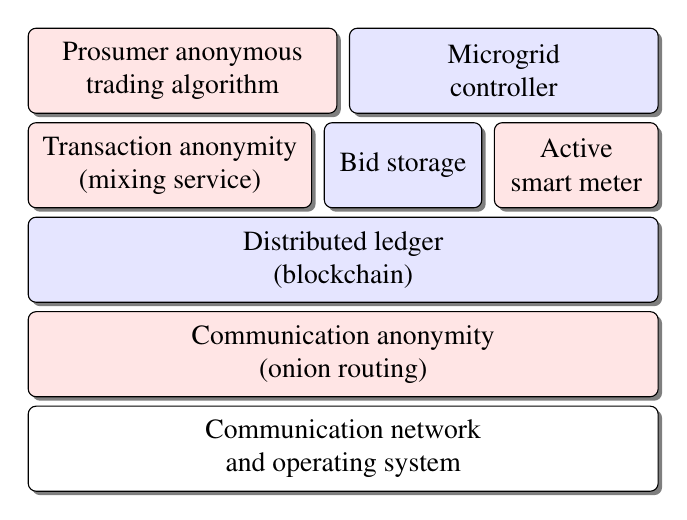
\begin{tikzpicture}[x=8cm, y=1.2cm,
  nodeStyle/.style={rounded corners=0.1cm, drop shadow={shadow xshift=0.05cm, shadow yshift=-0.05cm, fill=black}}
]
\draw [nodeStyle, fill=white]   (0, 0) rectangle    (1, 0.9) node [midway, align=center] {Communication network\\and operating system};

\draw [nodeStyle, fill=red!10]  (0, 1) rectangle    (1, 1.9) node [midway, align=center] {Communication anonymity\\(onion routing)};

\draw [nodeStyle, fill=blue!10] (0, 2) rectangle    (1, 2.9) node [midway, align=center] {Distributed ledger\\(blockchain)};

\draw [nodeStyle, fill=red!10]  (0,    3) rectangle (0.45, 3.9) node [midway, align=center] {Transaction anonymity\\(mixing service)};
\draw [nodeStyle, fill=blue!10] (0.47, 3) rectangle (0.72, 3.9) node [midway, align=center] {Bid storage};
\draw [nodeStyle, fill=red!10 ] (0.74, 3) rectangle (1,    3.9) node [midway, align=center] {Active\\smart meter};

\draw [nodeStyle, fill=red!10] (0,    4) rectangle (0.49, 4.9) node [midway, align=center] {Prosumer anonymous\\trading algorithm};
\draw [nodeStyle, fill=blue!10] (0.51, 4) rectangle (1,    4.9) node [midway, align=center] {Microgrid\\controller};
\end{tikzpicture}
\caption{High-level architecture of the proposed solution. Components marked red are introduced to provide privacy in a safe and secure manner. Components marked in blue are typical elements of a decentralized transactive microgrid.}
\label{fig:softwareArchitecture}
\end{figure}

\begin{figure*}[h]
\center
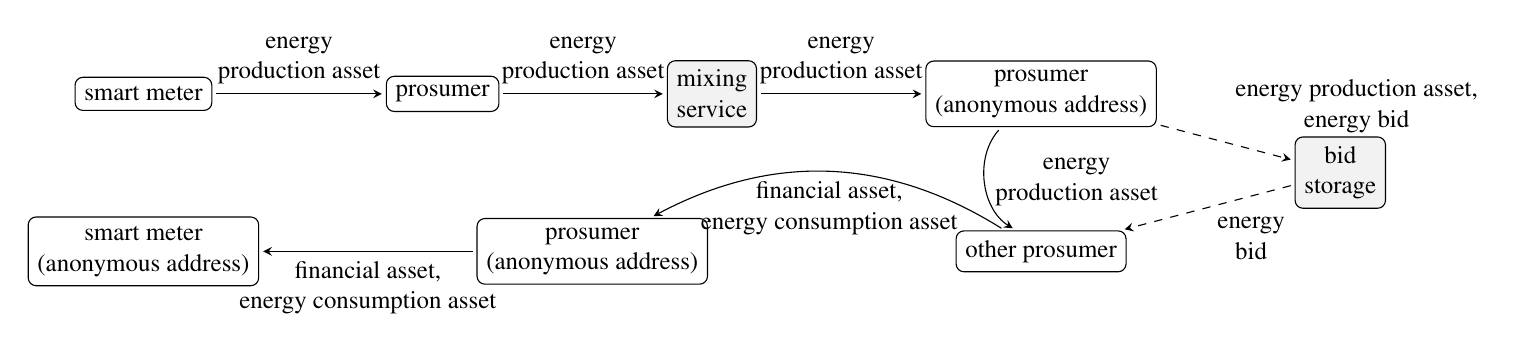
\begin{tikzpicture}[x=3.8cm, y=2cm, font=\small,
  system/.style={draw, align=center, rounded corners=0.1cm, fill=black!5},
  entity/.style={draw, align=center, rounded corners=0.1cm},
  asset/.style={midway, align=center},
  transfer/.style={->, >=stealth, shorten <=0.05cm, shorten >=0.05cm},
]
%\node[entity] (smartmeter) at (0.75, 0.5) {smart\\meter};
%\node[entity] (prosumer1) at (1.25, 1) {prosumer};
%\node[system] (mixing1) at (2, 1) {mixing\\service};
%\node[entity] (prosumer2) at (3, 1) {prosumer\\(alternative address)};
%\node[system] (bidstorage) at (4, 1) {bid\\storage};
%\node[entity] (partner) at (4, 0) {other prosumer};
%\node[entity] (prosumer3) at (3, 0) {prosumer\\(alternative address)};
%\node[system] (mixing2) at (2, 0) {mixing\\service};
%\node[entity] (prosumer4) at (1.25, 0) {prosumer};
\node[entity] (smartmeter) at (0, 1) {smart meter};
\node[entity] (prosumer1) at (1, 1) {prosumer};
\node[system] (mixing1) at (1.9, 1) {mixing\\service};
\node[entity] (prosumer2) at (3, 1) {prosumer\\(anonymous address)};
\node[system] (bidstorage) at (4, 0.5) {bid\\storage};
\node[entity] (partner) at (3, 0) {other prosumer};
\node[entity] (prosumer3) at (1.5, 0) {prosumer\\(anonymous address)};
\node[entity] (smartmeter2) at (0, 0) {smart meter\\(anonymous address)};

%\draw[transfer] (smartmeter) -- node [asset, above left] {energy\\production asset} (prosumer1);
%\draw[transfer] (prosumer1) -- node [asset, above] {energy\\production asset} (mixing1);
%\draw[transfer] (mixing1) -- node [asset, above] {energy\\production asset} (prosumer2);
%\draw[transfer, dashed] (prosumer2) -- node [asset, above] {energy production asset,\\energy bid} (bidstorage);
%\draw[transfer, dashed] (bidstorage) -- node [asset, right] {energy\\bid} (partner);
%\draw[transfer, bend right=15] (partner) to node [asset, below] {financial asset,\\energy\\consumption asset} (prosumer3);
%\draw[transfer, bend right=7.5] (prosumer2) to node [asset, above right] {energy\\prod. asset} (partner);
%\draw[transfer] (prosumer3) -- node [asset, below] {financial asset,\\
%energy consumption asset} (mixing2);
%\draw[transfer] (mixing2) -- node [asset, below] {financial asset,\\energy consumption asset} (prosumer4);
%\draw[transfer] (prosumer4) -- node [asset, below left] {financial\\asset} (smartmeter);

\draw[transfer] (smartmeter) -- node [asset, above] {energy\\production asset} (prosumer1);
\draw[transfer] (prosumer1) -- node [asset, above] {energy\\production asset} (mixing1);
\draw[transfer] (mixing1) -- node [asset, above] {energy\\production asset} (prosumer2);
\draw[transfer, dashed] (prosumer2) -- node [asset, above right] {energy production asset,\\energy bid} (bidstorage);
\draw[transfer, dashed] (bidstorage) -- node [asset, below right] {energy\\bid} (partner);
\draw[transfer, bend right=30] (partner) to node [asset, below] {financial asset,\\energy consumption asset} (prosumer3);
\draw[transfer, bend right=50] (prosumer2) to node [asset, right] {energy\\production asset} (partner);
\draw[transfer] (prosumer3) -- node [asset, below] {financial asset,\\
energy consumption asset} (smartmeter2);
\end{tikzpicture}
\caption{Simplified overview of the flow of assets from the perspective of a prosumer who sells energy. Note that in order to prevent de-anonymization, a prosumer should use multiple addresses and multiple rounds of mixing.}
\label{fig:sellFlow}
\end{figure*}

\subsection{Overview}
We begin with a semi-formal description of the energy trading process from the prosumers' perspective.
In subsequent subsections, we will describe the assets, transactions, and services in our system in more detail.

First, consider a prosumer who would like to sell energy to another prosumer (this case is illustrated in Figure~\ref{fig:sellFlow}).
As its very first step, the prosumer obtains an \emph{energy production asset} from its smart meter.
An energy production asset represents a permission to sell a certain amount of energy, and it is used to enforce safety requirements.
If the prosumer has sufficient unsold production capacity, the smart meter creates and transfers a production asset to the prosumer using a \emph{smart meter transaction}, which is recorded on the distributed ledger.

At this point, the production asset can still be traced back to the prosumer since the ledger is public.
To achieve anonymity, the prosumer transfers the production asset to a \emph{mixing service} using an \emph{energy and financial transaction}, which is also recorded on the distributed ledger.
In turn, the mixing service transfers the production asset to an \emph{anonymous address}\todo{We should probably insert a good definition here for reader who are unfamiliar with blockchain transactions.}, which is randomly generated and controlled by the prosumer.
Since the mixing service transfers assets from multiple prosumers to multiple anonymous addresses at the same time, and the anonymous addresses were chosen at random by the prosumers, the assets cannot be traced back to the original prosumers after mixing.\footnote{Note that prosumers should divide their assets between multiple anonymous addresses; otherwise, each asset might be traced back to its prosumer based on the amount of energy that it contains.}

Now, the prosumer can engage in energy trading anonymously.
To find a trade partner, it can either post an \emph{energy bid} on the bid storage, or simply search the storage for an acceptable \emph{energy ask}.
To post an energy bid, the prosumer first proves to the storage service -- without revealing its original identity -- that it owns a production asset stored at an anonymous address.
It can then post the energy bid, which contains an anonymous communication address\footnote{We discuss communication anonymity later.}, a price, and a reference to the production asset.
If another prosumer, who would like to buy energy, finds the bid acceptable, it can contact the selling prosumer at the communication address given by the bid.



\subsection{Timing}
The ability to specify points or intervals in time is crucial.
For example, control signals specify how the load should change at certain points in time, energy trades specify when energy will be consumed or produced, etc.
To facilitate processing signals and transactions, we divide time into fixed-length intervals, and specify points or periods in time using these discrete timesteps.
The length of the time interval is determined by mapping the timing assumptions of the power system to our platform.
%In our implementation, 
For example, the default length of the time interval may be 4 seconds, which corresponds to how frequently the control signal of the DSO typically changes.

\subsection{Services}

Here, we describe three services that must be implemented for our solution: communication anonymity, mixing service for transaction anonymity, and anonymous bid storage for bidding anonymity.

\subsubsection{Communication Anonymity}
Firstly, we must provide an anonymous communication layer, on which we can build an anonymous trading platform.
Without this communication layer, bids and transactions could be easily de-anonymized based on the network identifiers of the sources (e.g., IP or MAC addresses).

We can employ well-known and widely used techniques for anonymous communication, such as \emph{onion routing}.
To build an onion network, the smart meters, inverters, and other devices can act as onion routers, and the list of onion routers in a microgrid can be published on a private blockchain.
In our first implementation, we can use the free and open-source Tor software with private Directory Authorities.
% ritter.vg: "run your own tor network"
% https://ritter.vg/blog-run_your_own_tor_network.html

\subsubsection{Transaction Anonymity}
We must provide prosumers with the ability to create and publish transactions anonymously.
More specifically, prosumers should be able to purchase or sell energy without revealing their identity; however, these transaction must also be verifiable and enforceable.

We may achieve this goal using multiple approaches for blockchain transaction anonymity:
\begin{itemize}
\item Mixing services (also known as tumblers) mix potentially identifiable assets on a blockchain with others, thereby preventing tracing individual assets back to their original source. 
In our case, assets to be mixed include virtual balances of fiat currencies as well as energy production and consumption.
\item Cryptographic anonymity for transactions is provided, for example, by Zerocoin~\cite{miers2013zerocoin}. Similarly to mixing service, Zerocoin can prevent tracing assets on a blockchain.
\end{itemize}
Using the above techniques, we can enable prosumers to trade energy anonymously (i.e., without revealing their true identities), but at the same time prevent them from altering their energy or financial balances without a valid transaction.

However, we must also ensure that 1) smart meters know the amount of energy purchased or sold by their prosumer and 2) prosumers cannot purchase or sell more energy than their capacity.
To satisfy both of these constraints, all energy trades must start with the prosumer withdrawing a certain amount of energy production or consumption from its smart meter:
\begin{itemize}
\item If a prosumer wishes to sell energy, it must first obtain an energy asset from its smart meter using a blockchain transaction.
This transaction must be signed by the smart meter, which enables the smart meter to 1) keep track of the amount of energy traded by the prosumer as well as to 2) enforce safety requirements by limiting the amount of energy that can be withdrawn.
\item If a prosumer wishes to buy energy, it must first obtain an energy consumption asset from its smart meter in a way similar to obtaining an energy production asset.
\end{itemize}

\subsubsection{Bidding Anonymity}
Finally, we must provide prosumers with the ability to publish energy buy and sell bids anonymously.
To this end, we create a storage for anonymous bids that is readable by all the prosumers in the microgrid.
Any prosumer may submit a bid to this storage; however, in order to do so, they must provide a zero-knowledge proof of owning the assets that are to be traded:
\begin{itemize}
\item To submit an energy sell bid, the prosumer must prove that it owns an energy production asset on the chain.
\item To submit an energy buy bid, the prosumer must prove that it own an energy consumption asset as well as financial assets on the chain.
\end{itemize}


\subsection{Transaction Types}

Before we can discuss transaction types, we must first define the three assets that these transactions may transfer.

An \emph{energy production asset} (EPA) is defined by
\begin{compactitem}
\item \field{power}: non-negative amount of power to produced (for example, measured in watts).
\item \field{start}: first time interval in which energy is to be produced. 
\item \field{end}: last time interval in which energy is to be produced.
\end{compactitem}
An \emph{energy consumption asset} (ECA) is defined by the same fields; however, for this asset, the fields define consumption instead of production.
Finally, a \emph{financial asset} (FA) is defined by a single non-negative field \field{amount}, which can be denominated in either a fiat currency (e.g., US dollars) or a cryptocurrency.

\subsubsection{Energy and Financial Transactions}

Energy and financial transactions transfer energy and financial asset from one address to another.
Prosumers use these transactions for multiple purposes: to trade energy by exchanging assets with other prosumers, to prove to the bid storage that they have production or consumption capacity, to hide their identity by transferring assets to and from mixing services, and to deposit assets at their smart meter.
%
An energy and financial transaction contains the following fields:
\begin{compactitem}
\item List of EPA inputs, each of which is defined by:
\begin{compactitem}
\item \field{out}: EPA output from a previous transaction,
\item \field{sig}: signature for this output.
\end{compactitem}
\item List of ECA inputs, each of which is defined by:
\begin{compactitem}
\item \field{out}: ECA output from a previous transaction,
\item \field{sig}: signature for this output.
\end{compactitem}
\item List of FA inputs, each of which is defined by:
\begin{compactitem}
\item \field{out}: FA output from a previous transaction,
\item \field{sig}: signature for this output.
\end{compactitem}
\item List of EPA outputs, each of which is defined by:
\begin{compactitem}
\item an EPA and an address to which it is transferred.
\end{compactitem}
\item List of ECA outputs, each of which is defined by:
\begin{compactitem}
\item an ECA and an address to which it is transferred.
\end{compactitem}
\item List of FA outputs, each of which is defined by:
\begin{compactitem}
\item an FA and an address to which it is transferred.
\end{compactitem}
\end{compactitem}

An energy and financial transaction is valid if the following three conditions hold.
\begin{compactitem}
\item None of the outputs referenced by the inputs have been spent by a transaction that has been recorded on the ledger.
\item All of the signatures are valid.
\item For each asset type (and for each timestep), the sum of inputs and outputs is the same.
For example, in the case of energy production assets, the condition is:
\begin{align}
\forall t: & \sum_{out \in \text{EPA outputs}} out.\mathtt{power} \cdot 1_{\left\{out.\mathtt{start} \leq t \leq out.\mathtt{end}\right\}} \nonumber \\
& = \sum_{in \in \text{EPA inputs}} in.\mathtt{out}.\mathtt{power} \cdot 1_{\left\{in.\mathtt{out}.\mathtt{start} \leq t \leq in.\mathtt{out}.\mathtt{end}\right\}} ,
\end{align}
where $1_x$ is equal to $1$ if $x$ is true, and it is $0$ otherwise.
%\begin{equation}
%\forall t: \sum_{out \in \left\{out' \middle| out' \in \text{ EPA outputs} \wedge out'.EPA.start \leq t \leq out'.EPA.end\right\}} out.EPA.Power = \sum_{in \in \left\{in' \middle| in' \in \text{ EPA inputs} \wedge in'.EPA.start \leq t \leq in'.EPA.end\right\}} in.EPA.Power .
%\end{equation}
\end{compactitem}
If a transaction submitted to the ledger is valid, it will be permanently recorded.

\subsubsection{Smart-Meter Transactions}

Prosumers use smart-meter transactions to withdraw energy and financial assets from their own smart meters, before they engage in energy trading.
%
A smart-meter transaction contains the following fields:
\begin{compactitem}
\item List of EPA outputs, each of which is defined by:
\begin{compactitem}
\item an EPA and an address to which it is transferred.
\end{compactitem}
\item List of ECA outputs, each of which is defined by:
\begin{compactitem}
\item an ECA and an address to which it is transferred.
\end{compactitem}
\item List of FA outputs, each of which is defined by:
\begin{compactitem}
\item an FA and an address to which it is transferred.
\end{compactitem}
\item \field{id}: Identifier of the smart meter.
\item \field{sig}: Smart meter's signature over the transaction.
\end{compactitem}

A smart-meter transaction is valid if the following two conditions hold:
\begin{compactitem}
\item The smart meter identified in the transaction has been authorized by a regulatory transaction that has been recorded on the ledger.
\item The smart meter's signature is valid.
\end{compactitem}
\todo{To address malfunctioning or compromised smart meters, we could also impose a limit on withdrawals.}

\subsubsection{Regulatory Transactions}

The DSO uses regulatory transactions to authorize or ban smart meters and to control the microgrid load through setting a price policy.
Since these transactions provide a diverse set of functionality, they are divided into two types.

\paragraph{Authorize or Ban Smart Meters}
The DSO uses these transactions to manage the set of authorized smart meters in the microgrid.
Whenever a new smart meter is installed, the DSO notifies the members of the microgrid using a regulatory transaction.
Similarly, whenever a smart meter is deactivated (e.g., because service is stopped or it is believed to be malfunctioning or compromised), the DSO notifies the members of the microgrid using a regulatory transaction.
These transactions contain the following fields:
\begin{compactitem}
\item List of smart meters to be authorized, each of which is defined by:
\begin{compactitem}
\item \field{id}: Identifier of the smart meter.
\item \field{pubkey}: Public key of the smart meter.
\end{compactitem}
\item List of smart meters to be banned, each of which is given using its identifier.
\item \field{time}: Timestep in which smart meters are authorized and banned.
\item \field{sig}: DSO's signature over the transaction.
\end{compactitem}

A regulatory transaction of this type is valid if the following two conditions hold:
\begin{compactitem}
\item The timestep specified in the transaction is in the future.
\item The DSO's signature is valid.
\end{compactitem}

\paragraph{Price Policy}


%!TEX root = paper.tex
% \subsection{Services}\label{Services}

% We now describe the various services that are provided in PETra.
% Earlier, we discussed the distributed ledger, which permanently
% stores valid transactions.  Below, we introduce the anonymous
% communication service, the mixing service for transaction anonymity,
% the anonymous bid storage, and smart-meter based billing.

\subsection{Communication Anonymity}
\label{comm} 
The anonymous communication layer is the infrastructure upon which all
other anonymity services in PETra are built.  The goal of communication anonymity is to allow smart meters and users to exchange transactions and bids without revealing their IP-addresses or other information which can be used to identify them. In almost all cases, at the very least the Internet Service Provider (ISP) has information about the users' communications and identities. The goal of this section is to maximize the anonymity to such an extent that not even ISPs can identify users. Existing protocols for low-latency communication anonymity include onion routing ~\cite{reed1998anonymous} or the similar garlic routing \cite{Liu2014EmpiricalMA}, STAC \cite{7986314} and the decentralized Matrix protocol.\footnote{Open-federated protocol for instant messaging, Voice-over-IP and IoT communications (\url{https://matrix.org/}).} In this section, we present a brief survey of onion and garlic routing, especially with respect to application in PETra.

% \begin{figure}
%  \centering
%  \includegraphics[width=0.6\columnwidth]{onionrouting.png}
%  \caption{Conceptual visualization of onion routing between smart meters to secure communication anonymity. In the figure, smart meter A is sending a message m, with final destination B, through the onion routers.}\label{fig:onionrouting}
%  \end{figure}
 
\subsubsection{Onion and Garlic Routing}
Onion routing is based on messages in communication being encapsulated in multiple layers of encryption and sent through a number of nodes in a network, called onion routers. It is anonymous because no single node, except for the sender and the receiver, can know the origin and the recipient of the message. In Figure \ref{fig:garlicrouting}, an example shows how smart meter A encrypts a message $m$, with final destination G, through a network of onion routers. A encrypts the message, for example a confirmation of an energy purchase, a certain number of times, along with addresses of members of the onion network. Each subsequent node, selected by the sender and specified in the different layers of encryption, decrypts one layer using its private key, revealing the next node to which the encrypted message is forwarded. Finally, the second to last node reveals the address of smart meter G and sends the still encrypted message to G, who can decrypt it safely. No single node in the network, except for the sender, knows how many times the packages is re-routed, and no node except for the sender and recipient can know their internal position in the chain of routing. Another technique for communication anonymity is called \textit{garlic routing}. It differs from onion routing in that multiple messages are encrypted together to counter tracing attacks.

\begin{figure}
\centering
\includegraphics[width=\columnwidth]{garlicrouting.png}
\caption{The principle behind onion and garlic routing. The difference being that in onion routing, \textit{m} is a single message, whereas in garlic routing, \textit{m} is multiple messages packaged together.}\label{fig:garlicrouting}
\end{figure}

In practice, the deployment of onion routing (or a variant thereof called garlic routing) in the Invisible Internet Project (I2P) works as follows. Each node in the network operates an I2P router, allowing for anonymous communications. A router is distinct from an endpoint application in that it is not a secret who runs a router. By contrast, an application is the destination for the communications and is anonymous.  This disconnect allows for a higher degree of anonymity. To communicate between routers, unidirectional tunnels are set up. The tunnels use layered encryption, meaning that each router in the tunnel only can decrypt one layer. In order to transmit a message between two routers, the sender needs to know  where to direct the message, i.e. what the address of the entry point of the receiver is. 

The I2P protocol differs from regular network communications in that, for communications to take place between routers, each router needs to know a structure called the \textit{RouterInfo}. It contains the 2048-bit ELGamal encryption key, a signing key, a certificate, timestamp, text field, signature of bundle and the contact addresses where a router can be reached. The RouterInfo is given along with something called a \textit{LeaseSet}, containing a group of tunnel entry points for a particular client destination, when the tunnel will expire, the destination itself, encryption key for end-to-end encryption of garlic messages, revocation key and a signature of the LeaseSet data. The LeaseSet identifies an application on the I2P network. The I2P protocol ensures the anonymity of its users because of the disconnect between the identities of the applications communicating over the network, and the identities of the routers. This metadata is stored in a distributed directory called the netDb, based on the Kademlia P2P-protocol, which describes a provably consistent and fault-tolerant distributed hash table. \cite{kademlia} The RouterInfo and LeaseSet data are stored on the netDb under the key derived from the SHA256 of the destination.


\subsubsection{Threat Vectors in Onion and Garlic Routing}
\label{commthreat} 
	Murdoch and Danezis \cite{1425067} show that a low-cost traffic analysis is possible of the Tor-network, theoretically and experimentally. Traffic analyses are based on tracking the forwarding of the size of a data package between computers, for example, if computer A sends a package of exactly 42 bytes to computer J, who then sends a package of exactly 42 bytes to B, it can be easily deduced that A sent a package of unknown content to computer B. This is possible because of the distribution of metadata to all routers in the Tor-network~\cite{Hopper:2010:MAN:1698750.1698753}. In what is called a timing analysis attack, an attacker tries to find a correlation between the timing of messages moving through the network to gain information about user identities and their communications. Analyses have shown that these types of attacks can be very effective over a wide range of network parameters when specific defences are not employed~\cite{Levine2004,4797313}.  To counter timing analysis attacks, the I2P network bundles multiple messages together (principle of garlic routing) and renders it more difficult to analyse~\cite{Liu2014EmpiricalMA}. Schimmer, 2009, showed that the bandwidth opportunistic peer-selection and -profiling algorithm does not prioritize anonymity in favor of performance~\cite{peerProfiling:2009}. Herrmann and Grothoff, 2011, exposed a potential weakness in anonymous HTTP-hosting done over the I2P network \cite{Herrmann2011}. The arguably only practical attack against the I2P network was done against the directory, the netDb, by Egger \textit{et al.} \cite{Egger2013}. An improvement of the protocol, aimed at Egger \textit{et al.}'s attack was suggested by Timpanaro \textit{et al.}, 2015 \cite{Timpanaro2015}. 
    
Another potential weakness of onion routing and garlic routing is that, even though the actual message is encrypted and the destinations are unknown, there is always a trace of the communication at the ISP level. The fact that a connection took place will be logged and is openly visible at the very least to the ISP. This attack can be countered in PETra by each node transacting and participating in the mixing network, regardless of the need for trading at that time. Trading of ``zero''-assets can help obfuscate the non-zero-assets of others. Another liability in onion and garlic routing can be that the legitimacy of the sender can not be immediately verified. This can be achieved by the techniques described in the section Transaction Anonymity.  


 
\subsubsection{Proposed Solution}
Given the survey of the previous paragraphs, performing P2P energy trading in transactive grids over a garlic routing network protocol such as the I2P network provides a high amount of communication anonymity for users. Only part of the energy trading in PETra will be anonymized by garlic routing, namely the internet connections. PETra is no different from other network communications in that aspect. The particularity of the trading being local and thus IP-addresses being close, is a potential weakness that can be countered by creating ``fake'' IP-addresses. To apply garlic routing to transactive microgrids, the smart meters, prosumers, and DSO can act as onion routers, and distribution of available routers is done over netDb. In practice, this service
can be built on the free and open-source I2P software
 with private
Directory Authorities.  In this case, anonymous communication
identifiers in bids and asks correspond to public-keys that identify
I2P applications.
% ritter.vg: "run your own tor network"
% https://ritter.vg/blog-run_your_own_tor_network.html




\subsection{Transaction Anonymity}
\label{trans}
Communication anonymity is necessary but not sufficient for
anonymous trading, as the cryptographic objectives of authentication and legitimacy are not fulfilled. We suggest using cryptographic techniques from distributed ledgers, \textit{blockchains} and cryptocurrencies. The most adopted of which is the Bitcoin blockchain and currency. It allows for very simple digital cash spending but has serious privacy and anonymity flaws~\cite{Barber2012,Reid2013,apostolaki2017}. Additionally, Biryukov and Pustogarov, 2015, show that using Bitcoin over the Tor network opens an entirely new attack surface~\cite{biryukov2015}. Solutions to the tracing and identification problems identified by these researchers have been proposed and implemented in alternative cryptocurrency protocols: mixing using ring signatures and zero-knowledge proofs.~\cite{miers2013zerocoin,cryptonote} 

\subsubsection{Mixing Through Ring Signatures}
The CryptoNote protocol prevents tracing assets back to their original owners by
mixing together multiple incoming transactions and multiple outgoing
transactions. This service thus hides the connections between the
prosumers and the anonymous addresses. Mixing requires the possibility to create new wallets at will, something that is generally recommended upon any cryptocurrency transfer and it requires the existence of a sufficient number of participants in the network. These protocols enable participants to
mix assets with each other, thereby eliminating the need for a trusted
third party. Monero is an example of a cryptocurrency that provides built-in mixing services by implementing the CryptoNote protocol.~\cite{cryptoeprint:2015:1098} There are however alternative implementations of mixing protocols such as CoinShuffle~\cite{ruffing2014coinshuffle} or
Xim~\cite{bissias2014sybil}.

The CryptoNote protocol achieves two objectives:  
\begin{compactenum}
\item Untraceable transactions - \textit{for each incoming transaction all possible senders are equiprobable}. 
\item Unlinkable transactions - \textit{for any two outgoing transactions it is impossible to prove they were
sent to the same person}~\cite{cryptonote}.
\end{compactenum}

Group signatures were first introduced by Chaum and van Heyst, 1991,~\cite{Chaum1991} and then built upon by Rivest \textit{et al.}, 2001.~\cite{Rivest2001} The basis for anonymity in the CryptoNote protocol, however, is a slightly modified version of the \textit{Traceable ring signature} algorithm by Fukisaki and Suzuki, 2007.~\cite{Fujisaki2007} The algorithm allows a member of a group to send a transaction in such a way that it is impossible for a receiver to know any more about the sender than that it came from a group member without the use of a central authority.

Unlinkability is achieved by \textit{one-time ring signatures}, making use of four algorithms: \textbf{GEN, SIG, VER, LNK}. The general principle of the unconditional unlinkability is that a sender signs a transaction using a public key and a key image generated by \textbf{GEN} and produces a one-time ring signature using \textbf{SIG} and the public key pair and key image. \textbf{SIG} makes use of a non-interactive zero-knowledge proof which the verifier(s) then use to check the signature in \textbf{VER}. If the signature is valid, the verifier checks if the key image has been used in previous transactions, which mean that the same secret key was used to produce multiple signatures. She does that by running the algorithm \textbf{LNK}. Assuming that the mapping of the secret key to the key image is a one-way injection, it is certain that: \textbf{A.} The signer is not identifiable by way of recovering the secret key from the key image. \textbf{B.} The signer cannot create another key image with the same secret key. 

Additionally, if the receiver and sender have randomly generated, unique and new addresses, the Diffie-Hellman protocol can be used to generate a new pair of public-private keys. This is how untraceability of public keys is achieved. The sender should generate ephemeral keys for each transfer, enabling only the receiver to recover the corresponding private key. As an illustrative example, in Figure \ref{fig:ringsigs}, a schematic diagram shows households A, B and C signing a transaction since they are part of the same ring. A ring would, in reality, be many more households, not necessarily of the same microgrid. Let's assume that A is the true origin of the transaction. When E receives the transaction, the only thing that E can know with certainty is that one of A, B or C initiated the transaction. To increase the transaction anonymity further, a second, third or n rounds of ring signatures can be algorithmically imposed upon the network. With each round of signing parties, the group of potential origins grows linearly. Notably, the ring signature algorithm by Fujisaki and Suzuki, \cite{Fujisaki2007}, has been published in a peer-reviewed paper. This can be compared favorably to many cryptocurrency protocols which are simply published as white papers without any formal review-process. \cite{cryptonote}
In practice, a transaction using the mixing service should be performed in the following way to ensure anonymity:


It is also possible for household A that it paid prosumer B for energy by either disclosing the random number used in the generation of the one-time public destination key used in that transaction to B. Or she can use any other kind of zero-knowledge protocol to prove she knows the random number. The ring signatures would also allow the auditing of transactions by, for example, the DSO. This would be achieved by prosumer B giving the tracking key or truncated address to the DSO, who would then be able to link all incoming transactions to B.

\subsubsection{Mixing through Zero-Knowledge Proofs}
Zero-knowledge proofs (ZKP) are ways for a person to prove the knowledge of some specific fact to a verifier, without actually having to disclose the knowledge. Blum \textit{et al.} provided non-interactive ZKPs (NIZK) in 1988 \cite{Blum:1988:NZA:62212.62222}, where the prover and verifier don't have to interact or communicate directly with each other. The Zerocoin protocol \cite{miers2013zerocoin} outlines a way how NIZKs can achieve the untraceability objective of the previous section and it ensures that no double-spending is allowed.\footnote{Each coin in the protocol is identified uniquely by a serial number.} Zerocoin is a protocol for the decentralized mixing of coins, so that they can not be traced, or \textit{tainted}. However, senders and destinations can still be identified.~\cite{miers2013zerocoin} Luckily, Zerocash~\cite{Sasson:2014:ZDA:2650286.2650810} extends the NIZK functionality to allow for anonymous transactions, anonymous balances and coins, improved performance of transactions and sending of assets to a receivers fixed address without action required from the receiver. Zerocash makes use of a more efficient version of the NIZK, used in Zerocoin, called ZK \textit{Succinct Non-interactive ARguments of Knowledge} (zk-SNARK). 
% It features the algorithms: \textbf{Setup($1^\lambda$)}$\rightarrow \textit{params}$, \textbf{Mint(}\textit{params})$\rightarrow \textit{(c,skc)}$, \textbf{Spend}(\textit{params, c, skc, R, \textbf{C}})$\rightarrow(\pi, S)$ and \textbf{Verify}(\textit{params, $\pi$, S, R, \textbf{C}})$\rightarrow$$\{$0,1$\}$. The \textbf{Setup} function takes a secret parameter and returns a global public set of parameters and description of the set of coins. It is only executed once in the lifetime of the scheme, and the authors of the protocol recommend the usage of a trusted party for this. \textbf{Mint} is used to create coins from the coin set, given the parameters. \textbf{Spend} and \textbf{Verify} are executed by a sender and a receiver, respectively at the beginning and end of each transaction.

The Zerocash-scheme could be carried out using a simple messaging board, but would not be safe in practice since information might be manipulated or the owner of said board might collude etc. Therefore, an immutable, decentralized data storage, governed by the consensus of its peers is required to assure the secure transmission of information. The blockchain provides such a structure. 
% \begin{enumerate}[noitemsep,topsep=-\parskip]
% \item A mints a new message by generating a new random serial number $S$ of value $V$ and commits to it.
% \item The commitment, $C$, is such that only the secret message $m$ can reveal $S$.
% \item A then mints a second message by generating a new serial number $S_m$ so that the commitment $C$ is decrypted by the message $m$. 
% \item A posts the commitments to a blockchain along with the corresponding value in cryptocurrency.
% \item B has sold energy during the last timeperiod with references ($m_i,\dots m_j$) and has thereby $j-i$ number of references to scan the blockchain for.
% \item To redeem the payment, B produces a ZKP $\pi$ for the following statements:
% \begin{enumerate}[noitemsep,topsep=-\parskip]
% \item B knows a tuple ($C$) from all valid commitments available and
% \item B knows the secret $m$ such that the commitment ($C$) opens to ($S$) 
% \end{enumerate}
% \item B can now post a 'spend'-transaction containing ($S,\pi$) on the blockchain.
% \item The other users verify $\pi$ and ensure that ($S$) didn't occur already in the history of transactions.
% \item If correct, then the blockchain protocol allows B to collect cryptocurrency of value $V$. 
% \end{enumerate}
% This requires B to know all references to energy transactions that are outstanding (and coming from prosumer B) to date, and to be able to compare them to the available, valid commitments. 

\subsubsection{Threats and weaknesses in Ring Signature- and Zero-Knowledge Proof-schemes}
\label{transthreat} 
\begin{figure}[t]
\centering
\includegraphics[width=\columnwidth]{ringsigs.png}
\caption{Visualization of untraceability in ring signatures in smart meter-based energy trading and the potential deductions of origin of the transaction by a single household in the chain of signatures.}\label{fig:ringsigs}
\end{figure}
When applying either ring signatures or zero-knowledge SNARKs to PETra, potential weaknesses or attacks need to be considered.A potential threat to ring signatures is when a large amount of the unspent transactions are owned by an adversary or when insufficient amounts of signatures are included in a ring. When a prosumer A wishes to select a group of signatures to sign her transaction as well, then it is likely that she will select many of the transactions from the adversary. Assuming the adversary spends his outputs without \textit{mixing}\footnote{The number of other signatures used in the ring.}, then A's transaction is exposed as well.~\cite{monero2014} Recent research  also show that up to 65\% of Monero transactions are trivially traceable using one attack. They also exposes two more attacks that have been amended in the latest versions of the protocol, lowering the amount of transactions traceable to 20\%.~\cite{monero2014,DBLP:journals/corr/MillerMLN17} 

One of the main weaknesses of the Zerocash-based protocol is that for each private transaction, a costly zk-SNARK needs to be computed. But that is not a threat to anonymity, just a practical reason why it might be difficult to run the scheme over a congested public blockchain. In \cite{Sasson:2014:ZDA:2650286.2650810}, experiments show an average time of 3 min to create the zk-SNARK for a private transaction, verifying it takes only 8.5 ms. Another large practical drawback of Zerocash is the lack of programmability and functionality that would be required in PETra. Zhang \textit{et al.} solve some of the practical flaws and amend security issues.~\cite{zhangz} 

\subsubsection{Proposed Solution to Achieve Transaction Anonymity}
Applying the CryptoNote protocol to PETra could be done by performing both energy transactions and monetary transactions using ring signatures. They would be securely logged, tamper-proof and anonymous through the usage of a blockchain. Even though  some security flaws exists, as seen in the previous paragraph, the risk of identification, linking or tracing of transactions can be minimized by imposing a high minimum number of signatures per transaction. We also propose to connect the global transaction networks to augment the number of transactions and thereby limit the chance of deduction by elimination.

Applying ZKPs to PETra would require that a smart meter can encrypt and sign a transaction, transmit a proof of it to the blockchain and thus the receiver of the payment, without having to reveal the actual amount of energy or cost incurred to anyone but the receiver. This is achieved by the Zerocash-protocol and is implemented as a fork of the Bitcoin blockchain. Neither the receiver, nor any other participants can gain information about the transactions sent over the blockchain. To provide full functionality for PETra, the Zerocash-protocol would need to be implemented for the transmission of bids and asks as well as the already existing monetary transactions. The second implementation would need to be modified to transmit and link bids and asks to the payments ledger. A more straightforward but bloated structure would be to create transactions without monetary value to post a bid or an ask and then directly reference the final bid-/ask-transaction in the payment-transaction. 
% \subsubsection{Bidding Anonymity}
% Prosumers must also be able to anonymously post energy bids and asks
% on the bid storage service.  An anonymous bid (or ask) contains an ECA
% (or EPA), a price, and an anonymous communication identifier
% (\emph{e.g.}, Tor hidden service), which can be used to contact the
% bidding (or asking) prosumer.  To enforce safety requirements, the bid
% storage service must verify that the prosumer actually owns the asset
% to be traded.  To this end, the prosumer first has to prove that it
% controls the anonymous address where the asset is stored, which can be
% performed in multiple ways.

% In many distributed ledgers, an address represents a public key, and
% controlling means knowing the corresponding private key.  In this
% case, the prosumer can prove that it controls an address by signing a
% challenge, which was freshly generated by the service, with the
% private key of the address.

% \subsubsection{Smart-Meter Based Billing}
% After a prosumer has finished trading, it deposits all of its EPA,
% ECA, and FA to the smart meter by transferring them to an anonymous
% address generated by the smart meter.  Later, during timeslot $t$, the
% smart meter measures the amount of energy actually consumed (or
% produced) by the prosumer using physical sensors.  The meter can then
% compute the prosumer's bill for timeslot $t$, which will be paid to
% the DSO, as follows. \Abhishek{The safety argument should be
%   strengthened here}

% Notice that consumption assets are not used directly for billing, they are only used to enforce security and safety requirements.



%!TEX root = paper.tex



\section{Conclusion and Discussion}
\label{sec:discussion}

% This section presents an analysis of PETra and shows that
% it satisfies the security, safety, and privacy requirements formulated
% earlier.

% \subsection{Security}
% Satisfaction of the security requirements follows from:
% \begin{itemize}[noitemsep,topsep=-\parskip]
% \item immutability of transactions in the distributed ledger,
% \item validity of transactions
% \item and tamper-resistance of smart meters.
% \end{itemize}
% Together, these properties ensure that only the right entities may
% create and sign a transaction, that transactions adhere to the rules
% of the trading workflow, and that transactions cannot be tampered
% with. Double-spending is resolved by scanning the blockchain to allow only unique outputs. 

% \subsection{Safety}
% We now demonstrate that faulty or malicious prosumers cannot trade
% excessive amounts of energy if normal prosumers follow the rules of
% the trading workflow.  Due to the rules of the trading workflow, the gross amount of energy sold is less than or equal to the amount of EPA
% obtained by a prosumer.
% %
% A prosumer can obtain EPA either by withdrawing from its smart meter
% or by purchasing from another prosumer.  From its smart meter,
% prosumer can withdraw at most $\field{MAXEPA}$.  Although the
% prosumer may also buy EPA from another prosumer, this constitutes
% buying energy, which decreases the net amount of energy sold with the
% same amount.  Hence, the net amount of energy sold by prosumer
% cannot exceed $\field{MAXEPA}$.  By extending the argument, we can
% show that the net amount of energy sold by a group of prosumers~$G$
% cannot exceed $\sum_{i \in G} \field{MAXEPA}_i$.  Similarly, %we can
% %show that
%  the net amount of energy bought by a group of prosumers $G$
% cannot exceed $\sum_{i \in G} \field{MAXECA}_i$.

%Using a similar argument, we can also show that the total amount of energy bids (or asks) posted at
%the same time by prosumer $i$ for each timestep is at most
%$\field{MAXEPA}_i + \field{MAXECA}_i$.  This limit is higher than for
%net energy sold or bought, since prosumer $i$ may purchase
%$\field{MAXECA}_i$ amount of EPA (or $\field{MAXEPA}_i$ amount of ECA)
%from other prosumers, and then post an energy ask (or bid) in the
%amount of $\field{MAXEPA}_i + \field{MAXECA}_i$.

Through the use of garlic routing and ring signatures, complete communication and transaction anonymity is achieved. A garlic routing network such as I2P can ensure that no usage, bid, ask or identifiable data is leaked from the system. By using ring signatures, transactions cannot be traced, but it can still be proven that a bid or an ask has been responded to and that a transaction has taken place. The design we've proposed anonymizes the whole chain of transactions, both on a network communication layer and on a distributed ledger transaction layer.

As for the DSO, it receives the same information from the smart meter
as in a non-transactive smart grid (i.e., amount of energy
produced and consumed). In
particular, since price policies are recorded on the ledger (which the
smart meters may read), each prosumer's smart meter may calculate and
send the prosumer's monthly bill to the DSO, without revealing the
prosumer's energy consumption or production. The DSO still gets aggregate information regarding load on the grid, but cannot identify individual users and their energy prosumption. 





%!TEX root = paper.tex
\section{Related Work}
\label{sec:related}

%In this section we describe the related research. It has been divided into two subsections to focus on blockchains, which we are using to implement the distributed ledger service described earlier, and other works on smart grid privacy concerns. 

%\subsection{Smart Grid and Meter Privacy}
% http://ieeexplore.ieee.org/abstract/document/5054916/
%McDaniel and McLaughlin discuss privacy challenges in smart grids~\cite{mcdaniel2009security}.
% https://arxiv.org/pdf/1108.2234.pdf
% https://pdfs.semanticscholar.org/cdf8/a5b6256823bca38a1d2347ab36f8e4a2ca94.pdf
% http://www.comm.toronto.edu/~akhisti/sm.pdf
% https://www.researchgate.net/profile/Georgios_Kalogridis/publication/224189766_Smart_Grid_Privacy_via_Anonymization_of_Smart_Metering_Data/links/541169510cf2b4da1bec4193.pdf
% https://arxiv.org/pdf/1305.0735.pdf
New privacy concerns arise with the continuing adoption of smart
grids. In addition to old and new security threats (such as energy
theft and smart-meter malware), McDaniel and McLaughlin discuss the
privacy concerns of energy usage profiling that smart grids could
potentially enable~\cite{mcdaniel2009security}. Several approaches
have been investigated as potential means to provide privacy
protections for smart grid users.

Some approaches look to the use of protocols and/or frameworks to help
protect privacy. Rajagopalan et al.\ use tools from information theory
to present a framework that abstracts both the privacy and the utility
requirements of smart-meter
data~\cite{rajagopalan2011smart,sankar2013smart}. Their framework
leads to a novel tractable privacy-utility tradeoff problem with
minimal assumptions. Efthymiou and Kalogridis describe a method for
securely anonymizing frequent electrical metering data sent by a smart
meter~\cite{efthymiou2010smart}. Their approach is based on the
observation that frequent metering data may be required by an energy
distribution network for operational reasons, but it may not
necessarily need to be attributable to a specific smart meter. The
authors describe a method that provides a third-party escrow mechanism
for authenticated anonymous meter readings, which are hard to
associate with a particular smart meter.

Other approaches, such as additional hardware components, have also been explored 
for potential privacy gains. 
Varodayan and Khisti study using a
rechargeable battery for partially protecting the privacy of
information contained in a household's electrical load
profile~\cite{varodayan2011smart}. They show that stochastic battery
policies may leak 26\% less information than a best-effort policy,
which holds the output load constant whenever possible. Tan et
al.\ study privacy in a smart metering system from an information
theoretic perspective in the presence of energy harvesting and storage
units~\cite{tan2013increasing}. They show that energy harvesting
provides increased privacy by diversifying the energy source, while a
storage device can be used to increase both energy efficiency and
privacy.
% They show that there exists a trade-off between the information
% leakage rate and the wasted energy rate, and study the impact of the
% energy harvesting rate and the size of the storage device on this trade-off.

PETra extends this work by (1) leveraging a decentralized IoT
system for transactive energy and (2) addressing the novel privacy
threat posed by trading. In particular, while earlier work protected
the prosumers' privacy from the DSO, PETra also protects it from other
prosumers, as well as outside attackers.

A key element of PETra is its ability to distribute information among
peers via blockchains.  As blockchain technology develops and matures,
new frameworks, services, and protocols are being developed to
leverage the distributed ledgers provided by blockchains. For example,
Hyperledger Fabric is a platform for distributed ledger solutions,
which was designed to support pluggable implementations of different
components~\cite{hyperledger2017fabric}.
%Bitcoin Lightning Network is
%decentralized system, in which transactions are sent over a network of
%micropayment channels, whose transfer of value occurs
%off-blockchain~\cite{poon2016bitcoin}. 
Since this paper focuses on the theoretical foundations of PETra, any
of these distributed ledgers provide the required capabilities.

%\Abhishek{Aron this section should end with a few sentence about how our approach fits in. Perhaps just a few sentences reworded from introduction will be sufficient}

\iffalse
\subsection{Blockchains as Distributed Ledgers}

As Blockchain technology continues to develop and mature, new
frameworks, services, and protocols are being developed to leverage
blockchain's distributed ledger. Microsoft offers Blockchain as a
Service (BaaS) on Azure. Additionally, Microsoft has Project Bletchley
as its architectural approach to building an Enterprise Consortium
Blockchain Ecosystem, introducing two new concepts: blockchain
middleware and a secure means for calling code or data outside a
SmartContract or blockchain called
cryptlets~\cite{gray2016introducing}. Hyperledger Fabric is a platform
for distributed ledger solutions, which was designed to support
pluggable implementations of different
components~\cite{hyperledger2017fabric}. Bitcoin Lightning Network is
decentralized system, in which transactions are sent over a network of
micropayment channels whose transfer of value occurs
off-blockchain~\cite{poon2016bitcoin}. Interledger is a protocol for
payments across payment systems, which enables anyone with accounts on
two ledgers to create a connection between
them~\cite{thomas_protocol}. Xu et al.\ discuss the use of two pools
of proxy agents, an agreement pool and a payment pool, to assist in
protection of privacy when using blockchain technologies for
transactions on tangible goods~\cite{Xu2017}.  \fi

%\url{https://geli.net/residential/}
%\url{https://www.greentechmedia.com/articles/read/geli-raises-7m-to-take-energy-storage-software-to-the-next-level}

%\url{http://ethembedded.com/}


\section{Conclusion}
\label{sec:conclusion}

In this paper, we described the design and implementation of a  transaction management platform (TMP) for IoT-based transactive microgrids. Our solution enables prosumers to trade energy without threatening their privacy or the safety of the system. Our hybrid solver approach, which combines a smart-contract based validator with an external optimizer, enables the platform to clear offers securely and efficiently. Further, the ability to trade across multiple time intervals enables participants to take full advantage of batteries, thereby smoothening the load on the main grid. Finally, the use of blockchains provides decentralized trust and consensus capabilities, which protect from  malicious actors.


\AronC{future work:
- recovery from failures: retroactively change matching in case of a physical failure

- fault-tolerant matching: safety constraints will be satisfied even if a certain number of physical elements fail (or prosumers get disconnected)

- propose alternative market mechanisms, including those that involve double auctions and its variants.}




\section*{Acknowledgment}
This work was funded in part by a grant by Siemens Corporation, CT. 

% BALANCE COLUMNS
%\balance{}
%\setlength{\bibsep}{0pt plus 0ex}
%\let\oldthebibliography\thebibliography
%\let\endoldthebibliography\endthebibliography
%\renewenvironment{thebibliography}[1]{
%  \begin{oldthebibliography}{#1}
%    \setlength{\itemsep}{0.1em}
%    \setlength{\parskip}{0em}
%}
%{
%  \end{oldthebibliography}
%}

% REFERENCES FORMAT
% References must be the same font size as other body text.
\bibliographystyle{SIGCHI-Reference-Format}
\balance
\bibliography{references}

\end{document}

